% !TEX program = xelatex
\documentclass[11pt,a4paper]{article}

% ----------------------------------------------------------------------------------------
% Packages
% ----------------------------------------------------------------------------------------
\usepackage[top=1.5cm, bottom=1.5cm, left=2cm, right=2cm]{geometry} 
\usepackage{xeCJK}       % Chinese support (for names such as 中科第五纪)
\usepackage{titlesec}    
\usepackage{enumitem}    
\usepackage{hyperref}    
\usepackage{xcolor}      
\usepackage{fontawesome5} 
\usepackage{calc}
\usepackage{graphicx} 
\usepackage{tikz}      

% ----------------------------------------------------------------------------------------
% Font Settings
% ----------------------------------------------------------------------------------------
% English main font (default Latin Modern is fine under XeLaTeX).
% Chinese fonts — use Fandol (ships with TeX Live / MiKTeX by default).
\setCJKmainfont[BoldFont=FandolSong-Bold, ItalicFont=FandolKai-Regular]{FandolSong-Regular}
\setCJKsansfont[BoldFont=FandolHei-Bold]{FandolHei-Regular}
% If compiling locally on Windows without Fandol, you may replace the two lines above with:
% \setCJKmainfont{SimSun}

% ----------------------------------------------------------------------------------------
% Custom Formatting
% ----------------------------------------------------------------------------------------
\linespread{1.15} 

\titleformat{\section}
  {\Large\bfseries\raggedright} 
  {}{0em}                      
  {}                           
  [\titlerule]                 

\setlist[itemize]{leftmargin=*, parsep=0pt, itemsep=2pt, topsep=2pt}

% ----------------------------------------------------------------------------------------
% Document Start
% ----------------------------------------------------------------------------------------
\begin{document}

% ========================================================================================
% Header (Including Profile Picture)
% ========================================================================================
\noindent 
\begin{minipage}[t]{0.73\textwidth} 
    \vspace{0pt} 
    {\Huge\bfseries Yuze Zhu} \\[0.6em] 
    {\large
    \faUniversity\ University of Chinese Academy of Sciences, Beijing, China, 101408 \\[0.4em]
    \faEnvelope\ \href{mailto:zhuyuze23@mails.ucas.ac.cn}{zhuyuze23@mails.ucas.ac.cn} \quad | \quad
    \faPhone\ +86 155-5712-1756
    }
\end{minipage}%
\hfill 
\begin{minipage}[t]{0.23\textwidth} 
    \vspace{0pt} 
    \raggedleft 
    % Ensure the width is between 2.8cm and 3.0cm
    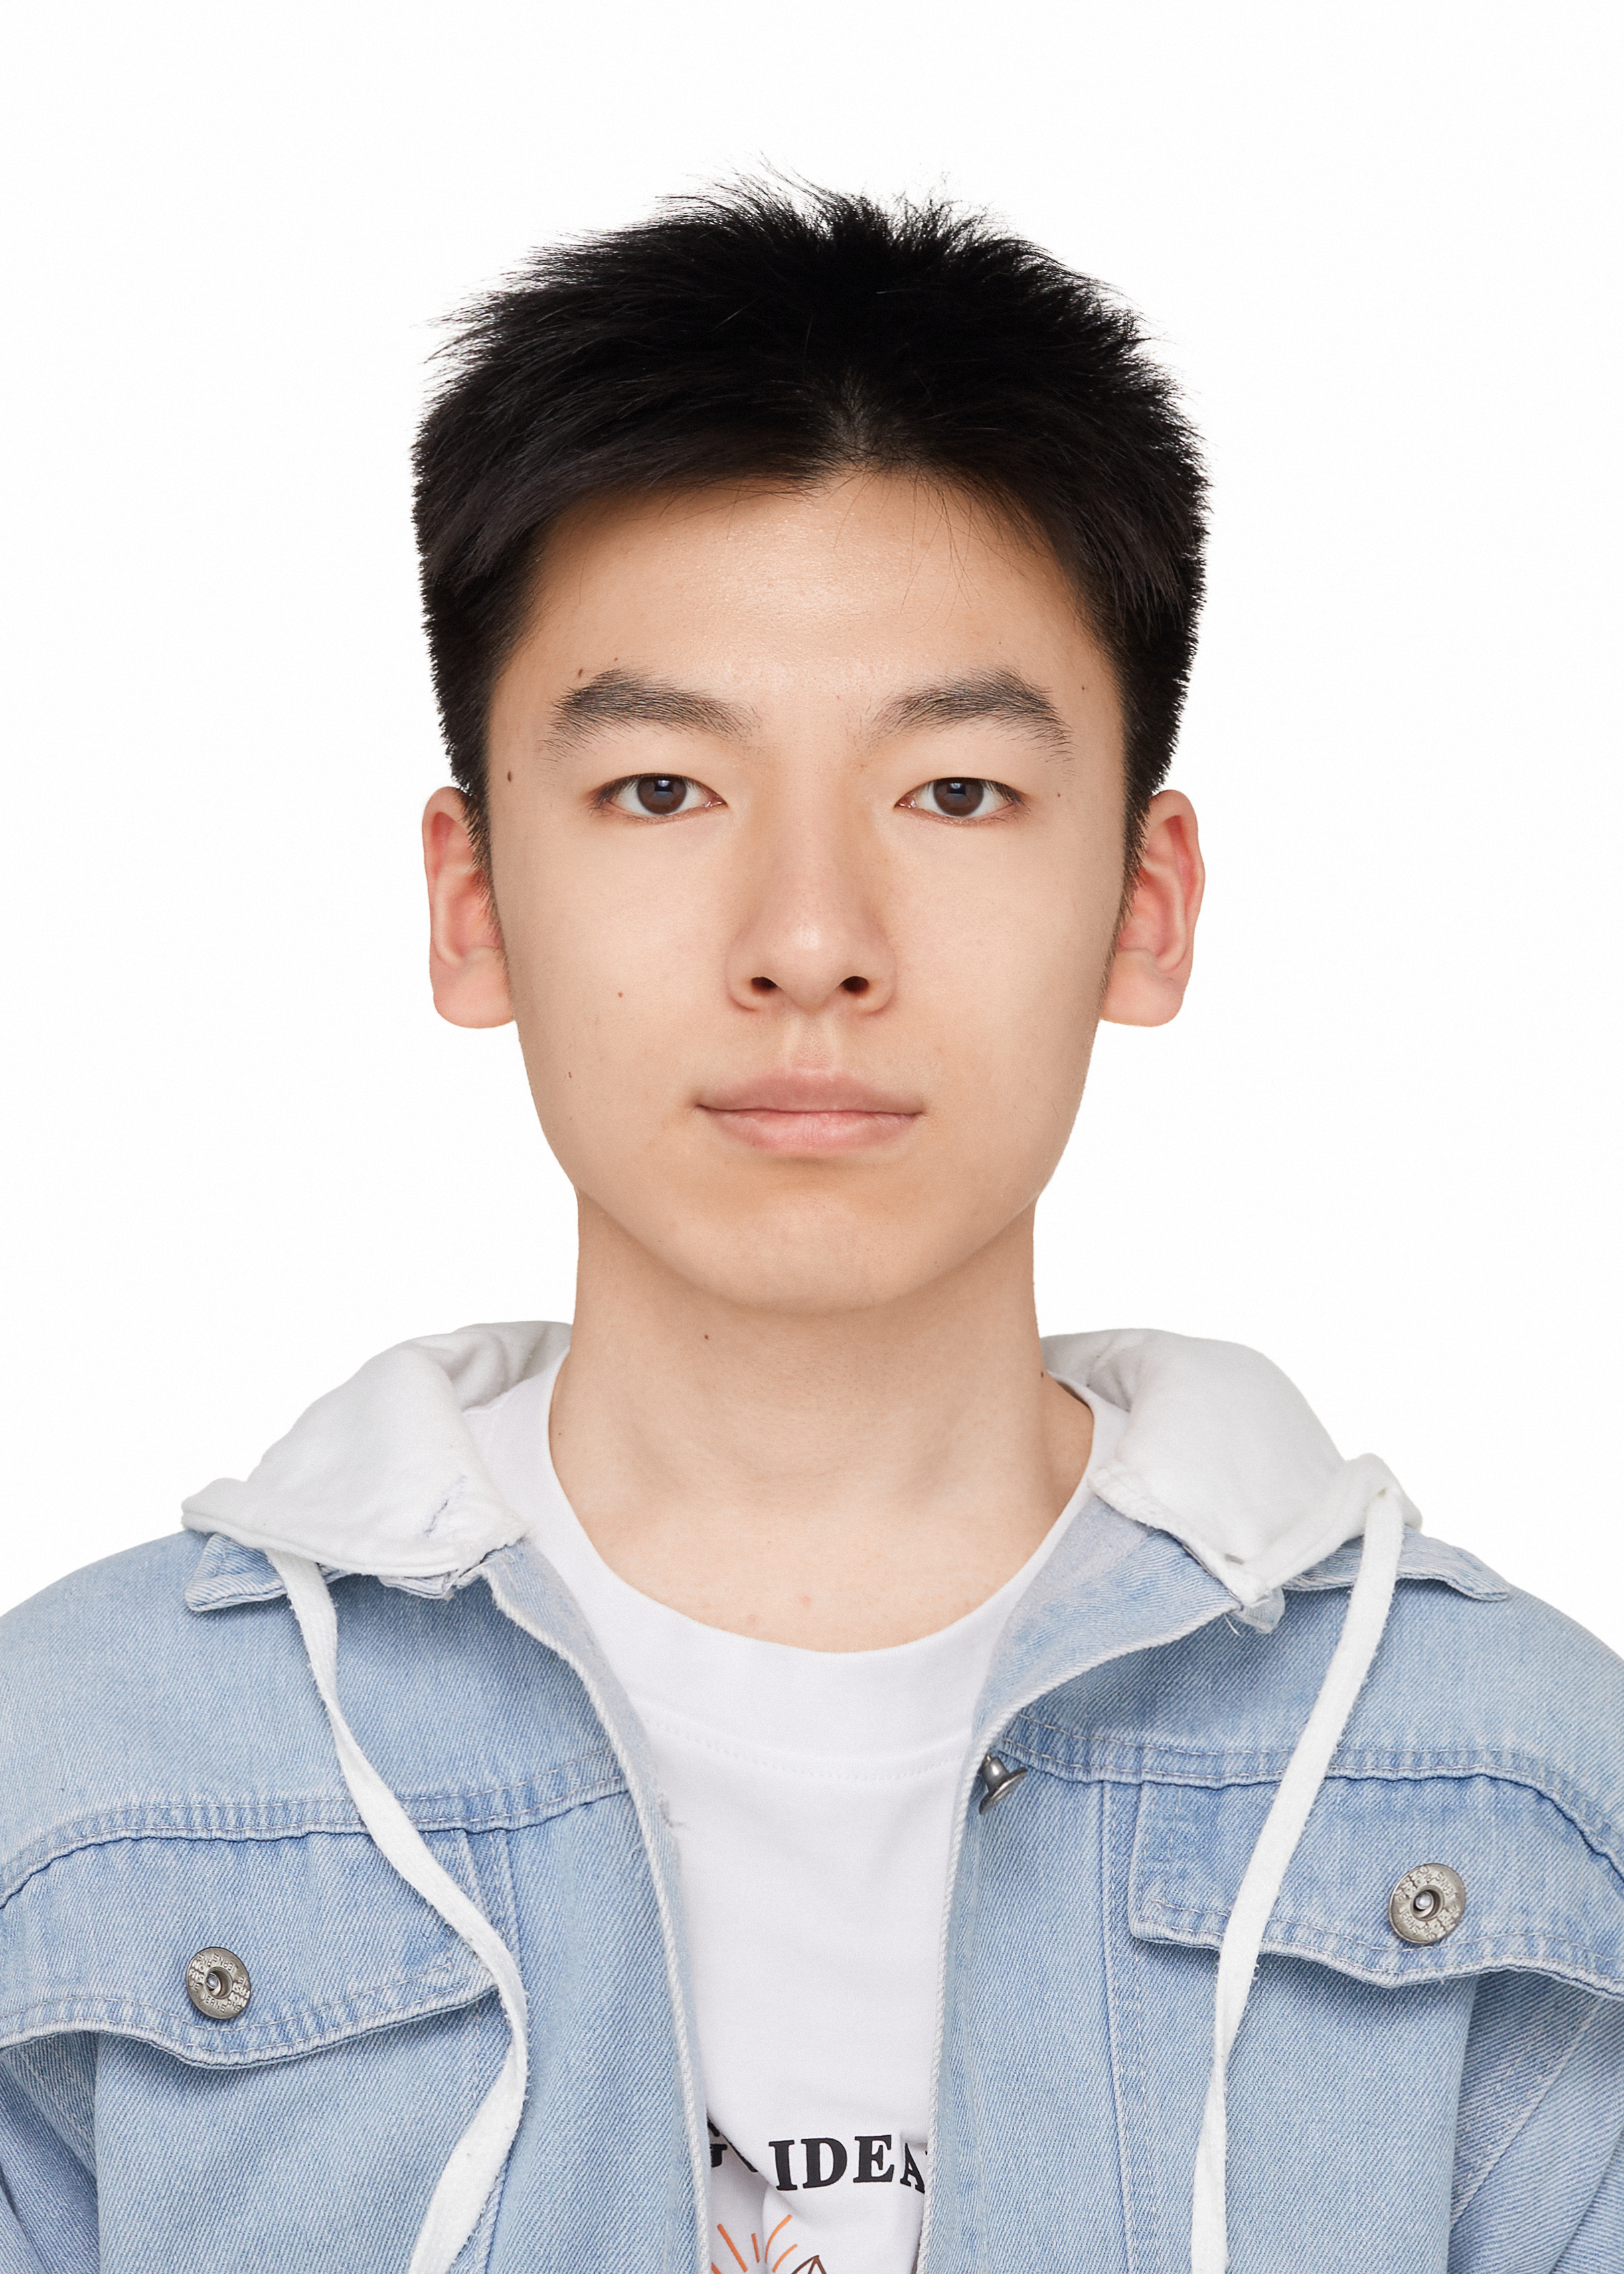
\includegraphics[width=2.8cm, keepaspectratio]{profile.jpg}
\end{minipage}

% ========================================================================================

% ----------------------------------------------------------------------------------------
% Education
% ----------------------------------------------------------------------------------------
\section{Education}
\textbf{University of Chinese Academy of Sciences (UCAS)} \hfill Beijing, China \\
\textit{B.Eng., School of Artificial Intelligence} \hfill Sep. 2023 -- Jul. 2027 (Expected)
\begin{itemize}
    \item \textbf{GPA:} 3.87 / 4.0 \quad \textbf{Rank:} 12/85 (Top 15\%)
    \item \textbf{Core Courses:} Computer Vision, Natural Language Processing, Robotics (Seminar), Pattern Recognition, Data Structures, etc.
\end{itemize}

% ----------------------------------------------------------------------------------------
% Experience
% ----------------------------------------------------------------------------------------
\section{Experience}
\textbf{FiveAges (中科第五纪)} \hfill Embodied AI Algorithm Intern \\
\textit{Embodied AI Algorithm Team, Beijing} \hfill Mar. 2026 -- Present \\
\textit{(Supervisor: Prof. Yan Huang)}
\begin{itemize}
    \item \textbf{Research Area:} Embodied intelligence algorithms, with a focus on \textbf{Vision-Language-Action (VLA)} models.
    \item \textbf{Core Work:} Contributing to the research and engineering of VLA models, and their deployment and verification on real-world robotic systems, bridging academic research with industrial applications.
\end{itemize}

\vspace{0.4em}
\textbf{Institute of Automation, Chinese Academy of Sciences (CASIA)} \hfill Research Intern \\
\textit{State Key Laboratory of Multimodal Artificial Intelligence Systems, Beijing} \hfill Jul. 2025 -- Jan. 2026 \\
\textit{(Supervisors: Assoc. Prof. Junyu Gao / Prof. Changsheng Xu)}
\begin{itemize}
    \item \textbf{Research Area:} Vision-Language Navigation (VLN) in Embodied AI, focusing on navigation mechanisms based on \textbf{self-correction}.
    \item \textbf{Core Contributions:} 
    \begin{itemize}
        \item Conceptualized an innovative method and detailed its implementation, proposing a novel dynamic path correction framework based on environmental feedback.
        \item Independently developed the \textbf{main experimental codebase}, conducted detailed \textbf{data analysis} and \textbf{ablation studies}, and quantitatively verified the contribution of each module.
        \item Conducted extensive comparative experiments on \textbf{R2R-CE} and \textbf{RxR-CE} (continuous environments) datasets, demonstrating that the proposed method effectively improves the navigation success rate.
    \end{itemize}
    \item \textbf{Outcome:} Co-authored a paper as the second author, submitted to the top-tier conference ICML 2026 (Under Review).
\end{itemize}

% ----------------------------------------------------------------------------------------
% Publications
% ----------------------------------------------------------------------------------------
\section{Publications}
\begin{itemize}
    \item Xuan Yao, \textbf{Yuze Zhu}, Junyu Gao, Zongmeng Wang, Changsheng Xu. ``\textit{[Title Anonymized for Double-Blind Review]}''. 
    \hfill \textbf{Submitted to ICML 2026 (Under Review)}
    \item \textit{Note: The specific paper title is omitted due to the ICML double-blind review process.}
\end{itemize}

% ----------------------------------------------------------------------------------------
% Course Project Experience
% ----------------------------------------------------------------------------------------
\section{Course Project Experience}
\textbf{Multimodal Polygraph System (Multimedia Information Processing)} \hfill Core Developer \\
\textit{Tech Stack: Python, Qwen3-VL, WavLM, Transformer} \hfill Oct. 2025 -- Dec. 2025
\begin{itemize}
    \item Aimed to achieve high-precision polygraphy by analyzing facial micro-expressions and speech features.
    \item Utilized the \textbf{Qwen3-VL} large model to extract high-dimensional visual and textual features, combined with \textbf{WavLM} for speech emotion features.
    \item Designed a multimodal feature concatenation network and classifier, achieving high recognition accuracy on the test set.
\end{itemize}

\textbf{MRI Reconstruction based on 3D Residual U-Net (Cognitive Neuroscience)} \hfill Algorithm Design \& Implementation \\
\textit{Tech Stack: PyTorch, Medical Image Processing, 3D CNN} \hfill Nov. 2025 -- Dec. 2025
\begin{itemize}
    \item Addressed the issue of low signal-to-noise ratio in low-field MRI images by exploring deep learning-based image enhancement methods.
    \item Built and trained a \textbf{3D Residual U-Net}, utilizing residual connections to accelerate convergence and preserve high-frequency details, successfully achieving high-quality reconstruction from low-field to high-field MRI.
\end{itemize}

\textbf{Remote-Controlled Robot Car Assembly and Control (Robotics Seminar)} \hfill Independently Completed \\
\textit{Tech Stack: Arduino, Sensors, Control Theory} \hfill Mar. 2024 -- Jun. 2024
\begin{itemize}
    \item Led hardware selection and assembly of the robot car, and debugged motor drivers and sensor modules.
    \item Developed control programs to implement basic obstacle avoidance and remote-control cruising functions.
\end{itemize}

% ----------------------------------------------------------------------------------------
% Honors & Awards
% ----------------------------------------------------------------------------------------
\section{Honors \& Awards}
\begin{itemize}
    \item \textbf{Second Prize Undergraduate Excellent Scholarship} (Top 15\% in Comprehensive Evaluation) \hfill 2024
    \item \textbf{Merit Student}, University of Chinese Academy of Sciences \hfill 2024
    \item \textbf{Merit Student}, University of Chinese Academy of Sciences \hfill 2023
\end{itemize}

% ----------------------------------------------------------------------------------------
% Extracurricular Experience
% ----------------------------------------------------------------------------------------
\section{Extracurricular Experience}
\textbf{``Chunfen Project'' Science Popularization Volunteer Program} \hfill Core Volunteer \hfill 2023 -- Present
\begin{itemize}
    \item \textbf{Science Lectures:} Delivered science outreach lectures at over ten primary schools in Beijing, featuring flame test demonstrations to spark scientific curiosity among students.
    \item \textbf{Content Creation:} Contributed to writing over \textbf{60 entries} for the ``Chunfen Project Science Encyclopedia'', translating complex concepts into accessible articles.
\end{itemize}

% ----------------------------------------------------------------------------------------
% Skills & Languages
% ----------------------------------------------------------------------------------------
\section{Skills \& Languages}
\begin{itemize}
    \item \textbf{Programming Languages:} Python (Proficient), C/C++, LaTeX
    \item \textbf{Frameworks / Tools:} PyTorch, HuggingFace, Linux, Git, Docker
    \item \textbf{Languages:} Chinese (Native), English (TOEFL 5.0/6.0, Fluent in academic reading and writing)
\end{itemize}

\end{document}